\documentclass[12pt,utf8,notheorems,compress,t]{beamer}
\usepackage{etex}

\usepackage{pgfpages}
\usepackage[export]{adjustbox}

% Workaround for the issue described at
% https://tex.stackexchange.com/questions/164406/beamer-using-href-in-notes.
\newcommand{\fixedhref}[2]{\makebox[0pt][l]{\hspace*{\paperwidth}\href{#1}{#2}}\href{#1}{#2}}

\usepackage[english]{babel}

\usepackage{graphbox}
\usepackage{mathtools}
\usepackage{booktabs}
\usepackage{stmaryrd}
\usepackage{amssymb}
\usepackage{array}
\usepackage{ragged2e}
\usepackage{multicol}
\usepackage{tabto}
\usepackage{xstring}
\usepackage{ifthen}
\usepackage[normalem]{ulem}
\usepackage[all]{xy}
\xyoption{rotate}
\usepackage{tikz}
\usetikzlibrary{calc,shapes,shapes.callouts,shapes.arrows,patterns,fit,backgrounds,decorations.pathmorphing,positioning}
\hypersetup{colorlinks=true}

\newcommand*\circled[1]{\tikz[baseline=(char.base)]{%
  \node[shape=circle,draw,inner sep=1pt] (char) {#1};}}

\DeclareFontFamily{U}{bbm}{}
\DeclareFontShape{U}{bbm}{m}{n}
   {  <5> <6> <7> <8> <9> <10> <12> gen * bbm
      <10.95> bbm10%
      <14.4>  bbm12%
      <17.28><20.74><24.88> bbm17}{}
\DeclareFontShape{U}{bbm}{m}{sl}
   {  <5> <6> <7> bbmsl8%
      <8> <9> <10> <12> gen * bbmsl
      <10.95> bbmsl10%
      <14.4> <17.28> <20.74> <24.88> bbmsl12}{}
\DeclareFontShape{U}{bbm}{bx}{n}
   {  <5> <6> <7> <8> <9> <10> <12> gen * bbmbx
      <10.95> bbmbx10%
      <14.4> <17.28> <20.74> <24.88> bbmbx12}{}
\DeclareFontShape{U}{bbm}{bx}{sl}
   {  <5> <6> <7> <8> <9> <10> <10.95> <12> <14.4> <17.28>%
      <20.74> <24.88> bbmbxsl10}{}
\DeclareFontShape{U}{bbm}{b}{n}
   {  <5> <6> <7> <8> <9> <10> <10.95> <12> <14.4> <17.28>%
      <20.74> <24.88> bbmb10}{}
\DeclareMathAlphabet{\mathbbm}{U}{bbm}{m}{n}
\SetMathAlphabet\mathbbm{bold}{U}{bbm}{bx}{n}

\usepackage{pifont}
\newcommand{\cmark}{\ding{51}}
\newcommand{\xmark}{\ding{55}}
\DeclareSymbolFont{extraup}{U}{zavm}{m}{n}
\DeclareMathSymbol{\varheart}{\mathalpha}{extraup}{86}

\graphicspath{{images/}}

\usepackage[protrusion=true,expansion=true]{microtype}

\setlength\parskip{\medskipamount}
\setlength\parindent{0pt}

\title{Revisiting divisible, injective and flabby abelian groups from a
constructive point of view}
\author{Ingo Blechschmidt}
\date{September ??th, 2022}

%\useinnertheme[shadow=true]
\setbeamerfont{block title}{size={}}

\useinnertheme{rectangles}

\usecolortheme{orchid}
\usecolortheme{seahorse}
\definecolor{mypurple}{RGB}{150,0,255}
\setbeamercolor{structure}{fg=mypurple}
\definecolor{myred}{RGB}{150,0,0}
\setbeamercolor*{title}{bg=myred,fg=white}
\setbeamercolor*{titlelike}{bg=myred,fg=white}
\setbeamercolor{frame}{bg=black}

\usefonttheme{serif}
\usepackage[T1]{fontenc}
\usepackage{libertine}

% lifted from https://arxiv.org/abs/1506.08870
\DeclareFontFamily{U}{min}{}
\DeclareFontShape{U}{min}{m}{n}{<-> udmj30}{}
\newcommand\yon{\!\text{\usefont{U}{min}{m}{n}\symbol{'210}}\!}

\newcommand{\A}{\mathcal{A}}
\newcommand{\B}{\mathcal{B}}
\newcommand{\C}{\mathcal{C}}
\newcommand{\M}{\mathcal{M}}
\renewcommand{\AA}{\mathbb{A}}
\newcommand{\BB}{\mathbb{B}}
\newcommand{\pp}{\mathbbm{p}}
\newcommand{\MM}{\mathbb{M}}
\newcommand{\E}{\mathcal{E}}
\newcommand{\F}{\mathcal{F}}
\newcommand{\FF}{\mathbb{F}}
\newcommand{\G}{\mathcal{G}}
\newcommand{\J}{\mathcal{J}}
\newcommand{\GG}{\mathbb{G}}
\renewcommand{\O}{\mathcal{O}}
\newcommand{\K}{\mathcal{K}}
\newcommand{\NN}{\mathbb{N}}
\newcommand{\QQ}{\mathbb{Q}}
\newcommand{\RR}{\mathbb{R}}
\newcommand{\TT}{\mathbb{T}}
\newcommand{\PP}{\mathbb{P}}
\newcommand{\ZZ}{\mathbb{Z}}
\newcommand{\CC}{\mathbb{C}}
\renewcommand{\P}{\mathcal{P}}
\newcommand{\aaa}{\mathfrak{a}}
\newcommand{\ppp}{\mathfrak{p}}
\newcommand{\fff}{\mathfrak{f}}
\newcommand{\defeq}{\vcentcolon=}
\newcommand{\defeqv}{\vcentcolon\equiv}
\newcommand{\Sh}{\mathrm{Sh}}
\newcommand{\GL}{\mathrm{GL}}
\newcommand{\Zar}{\mathrm{Zar}}
\newcommand{\op}{\mathrm{op}}
\newcommand{\Set}{\mathrm{Set}}
\newcommand{\Eff}{\mathrm{Ef{}f}}
\newcommand{\Sch}{\mathrm{Sch}}
\newcommand{\Aff}{\mathrm{Aff}}
\newcommand{\Ring}{\mathrm{Ring}}
\newcommand{\LocRing}{\mathrm{LocRing}}
\newcommand{\LRS}{\mathrm{LRS}}
\newcommand{\Hom}{\mathrm{Hom}}
\newcommand{\Spec}{\mathrm{Spec}}
\newcommand{\lra}{\longrightarrow}
\newcommand{\RelSpec}{\operatorname{Spec}}
\renewcommand{\_}{\mathpunct{.}}
\newcommand{\?}{\,{:}\,}
\newcommand{\speak}[1]{\ulcorner\text{\textnormal{#1}}\urcorner}
\newcommand{\ul}[1]{\underline{#1}}
\newcommand{\affl}{\ensuremath{{\ul{\ensuremath{\AA}}^1}}}
\newcommand{\Ll}{\text{iff}}
\newcommand{\inv}{inv.\@}
\newcommand{\seq}[1]{\mathrel{\vdash\!\!\!_{#1}}}
\newcommand{\hg}{\mathbin{:}}  % homogeneous coordinates

\setbeamertemplate{blocks}[rounded][shadow=false]

\newenvironment{indentblock}{%
  \list{}{\leftmargin\leftmargin}%
  \item\relax
}{%
  \endlist
}

% Adapted from https://latex.org/forum/viewtopic.php?t=2251 (Stefan Kottwitz)
\newenvironment<>{hilblock}{
  \begin{center}
    \begin{minipage}{9.05cm}
      \setlength{\textwidth}{9.05cm}
      \begin{actionenv}#1
        \def\insertblocktitle{}
        \par
        \usebeamertemplate{block begin}}{
        \par
        \usebeamertemplate{block end}
      \end{actionenv}
    \end{minipage}
  \end{center}}

\newenvironment{changemargin}[2]{%
  \begin{list}{}{%
    \setlength{\topsep}{0pt}%
    \setlength{\leftmargin}{#1}%
    \setlength{\rightmargin}{#2}%
    \setlength{\listparindent}{\parindent}%
    \setlength{\itemindent}{\parindent}%
    \setlength{\parsep}{\parskip}%
  }%
  \item[]}{\end{list}}

\tikzset{
  invisible/.style={opacity=0,text opacity=0},
  visible on/.style={alt={#1{}{invisible}}},
  alt/.code args={<#1>#2#3}{%
    \alt<#1>{\pgfkeysalso{#2}}{\pgfkeysalso{#3}}}
}

\newcommand{\pointthis}[3]{%
  \tikz[remember picture,baseline]{
    \node[anchor=base,inner sep=0,outer sep=0] (#2) {#2};
    \node[visible on=#1,overlay,rectangle callout,rounded corners,callout relative pointer={(0.3cm,0.5cm)},fill=blue!20] at ($(#2.north)+(-0.1cm,-1.1cm)$) {#3};
  }%
}

\tikzset{
  invisible/.style={opacity=0,text opacity=0},
  visible on/.style={alt={#1{}{invisible}}},
  alt/.code args={<#1>#2#3}{%
    \alt<#1>{\pgfkeysalso{#2}}{\pgfkeysalso{#3}}}
}

\newcommand{\hcancel}[5]{%
  \tikz[baseline=(tocancel.base)]{
    \node[inner sep=0pt,outer sep=0pt] (tocancel) {#1};
    \draw[red!80, line width=0.4mm] ($(tocancel.south west)+(#2,#3)$) -- ($(tocancel.north east)+(#4,#5)$);
  }%
}

\newcommand{\explain}[7]{%
  \tikz[remember picture,baseline]{
    \node[anchor=base,inner sep=2pt,outer sep=0,fill=#3,rounded corners] (label) {#1};
    \node[anchor=north,visible on=<#2>,overlay,rectangle callout,rounded corners,callout
    relative pointer={(0.0cm,0.5cm)+(0.0cm,#6)},fill=#3] at ($(label.south)+(0,-0.3cm)+(#4,#5)$) {#7};
  }%
}

\newcommand{\explainstub}[2]{%
  \tikz[remember picture,baseline]{
    \node[anchor=base,inner sep=2pt,outer sep=0,fill=#2,rounded corners] (label) {#1};
  }%
}

\newcommand{\squiggly}[1]{%
  \tikz[remember picture,baseline]{
    \node[anchor=base,inner sep=0,outer sep=0] (label) {#1};
    \draw[thick,color=red!80,decoration={snake,amplitude=0.5pt,segment
    length=3pt},decorate] ($(label.south west) + (0,-2pt)$) -- ($(label.south east) + (0,-2pt)$);
  }%
}

% Adapted from https://latex.org/forum/viewtopic.php?t=2251 (Stefan Kottwitz)
\newenvironment<>{varblock}[2]{\begin{varblockextra}{#1}{#2}{}}{\end{varblockextra}}
\newenvironment<>{varblockextra}[3]{
  \begin{center}
    \begin{minipage}{#1}
      \begin{actionenv}#4
        {\centering \hil{#2}\par}
	\def\insertblocktitle{}%\centering #2}
        \def\varblockextraend{#3}
	\usebeamertemplate{block begin}}{
        \par
        \usebeamertemplate{block end}
        \varblockextraend
      \end{actionenv}
    \end{minipage}
  \end{center}}

\setbeamertemplate{headline}{}

\setbeamertemplate{frametitle}{%
  \vskip0.5em%
  \leavevmode%
  \begin{beamercolorbox}[dp=1ex,center]{}%
    \begin{tikzpicture}
      \def\R{8pt}
      \node (title) {\hil{{\large\,\!\insertframetitle}}};
      \begin{pgfonlayer}{background}
        \draw[decorate, very thick, draw=mypurple!30]
          ($(title.south west) + (\R, 0)$) arc(270:180:\R) --
          ($(title.north west) + (0, -\R)$) arc(180:90:\R) --
          ($(title.north east) + (-\R, 0)$) arc(90:0:\R) --
          ($(title.south east) + (0, \R)$) arc(0:-90:\R) --
          cycle;
      \end{pgfonlayer}
    \end{tikzpicture}
  \end{beamercolorbox}%
  \vskip-0.2em%
}

\setbeamertemplate{navigation symbols}{}

\newcounter{framenumberpreappendix}
\newcommand{\backupstart}{
  \setcounter{framenumberpreappendix}{\value{framenumber}}
}
\newcommand{\backupend}{
  \addtocounter{framenumberpreappendix}{-\value{framenumber}}
  \addtocounter{framenumber}{\value{framenumberpreappendix}}
}

\newcommand{\insertframeextra}{}
\setbeamertemplate{footline}{%
  \begin{beamercolorbox}[wd=\paperwidth,ht=2.25ex,dp=1ex,right,rightskip=1mm,leftskip=1mm]{}%
    % \inserttitle
    \hfill
    \insertframenumber\insertframeextra\,/\,\inserttotalframenumber
  \end{beamercolorbox}%
  \vskip0pt%
}


\newcommand{\hil}[1]{{\usebeamercolor[fg]{item}{\textbf{#1}}}}
\newcommand{\bad}[1]{\textcolor{red!90}{\textnormal{#1}}}

\newcommand{\bignumber}[1]{%
  \renewcommand{\insertenumlabel}{#1}\scalebox{1.2}{\!\usebeamertemplate{enumerate item}\!}
}
\newcommand{\normalnumber}[1]{%
  {\renewcommand{\insertenumlabel}{#1}\!\usebeamertemplate{enumerate item}\!}
}
\newcommand{\bigheart}{
\includegraphics{heart}}

\newcommand{\subhead}[1]{{\centering\textcolor{gray}{\hrulefill}\quad\textnormal{#1}\quad\textcolor{gray}{\hrulefill}\par}}

\newcommand{\badbox}[1]{\colorbox{red!30}{#1}}
\newcommand{\grayline}{\textcolor{gray}{\hspace*{-3em}\hrulefill\hspace*{-3em}}}

\begin{document}

\addtocounter{framenumber}{-1}

%\setbeamertemplate{headline}{\mynav{gray}{gray}{gray}}

{\usebackgroundtemplate{\begin{minipage}{\paperwidth}\vspace*{4.95cm}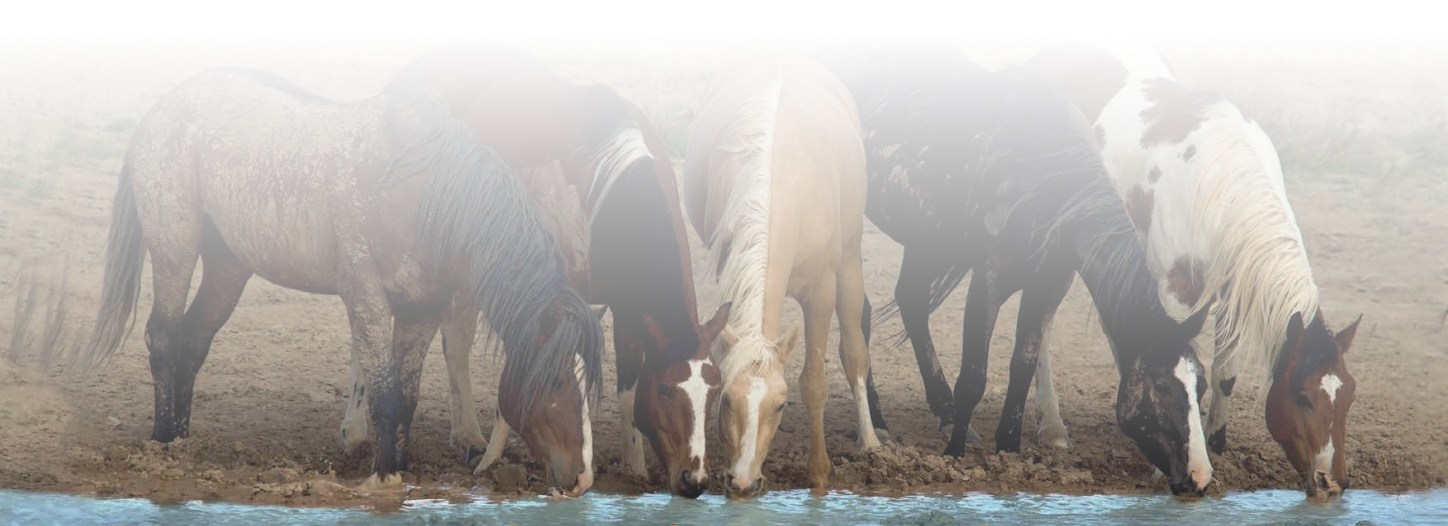
\includegraphics[width=\paperwidth]{topos-horses}\end{minipage}}
\begin{frame}[c]
  \centering

  \bigskip
  %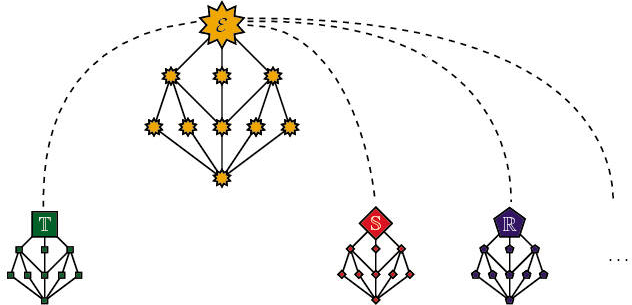
\includegraphics[height=0.32\textwidth]{olivia-lattices}
  \bigskip
  \bigskip
  \bigskip
  \bigskip

  \begin{tikzpicture}
    \def\R{8pt}
    \node (title) {\vbox{\vspace*{-0.0em}Revisiting divisible, injective and
    flabby abelian groups \\ from a constructive point of view\\[0.8em]}};
    \begin{pgfonlayer}{background}
      \draw[decorate, very thick, draw=mypurple]
        ($(title.south west) + (\R, 0)$) arc(270:180:\R) --
        ($(title.north west) + (0, -\R)$) arc(180:90:\R) --
        ($(title.north east) + (-\R, 0)$) arc(90:0:\R) --
        ($(title.south east) + (0, \R)$) arc(0:-90:\R) --
        cycle;
    \end{pgfonlayer}
  \end{tikzpicture}

  \scriptsize
  \textit{-- an invitation --}
  \bigskip
  \bigskip
  \bigskip

  REDCOM: \\
  \emph{Reducing complexity in algebra, logic, combinatorics}
  \ \\
  September ??th, 2022
  \bigskip

  Ingo Blechschmidt \\
  University of Augsburg
  \par
\end{frame}}

{\usebackgroundtemplate{\begin{minipage}{\paperwidth}\vspace{5.6cm}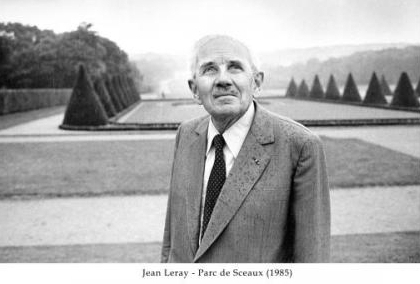
\includegraphics[width=\paperwidth]{leray}\end{minipage}}
\newcommand{\smallsphere}{\ensuremath{\vcenter{\hbox{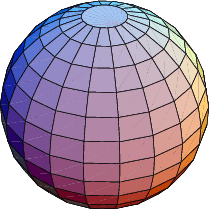
\includegraphics[height=1em]{sphere}}}}}
\newcommand{\smalltorus}{\ensuremath{\vcenter{\hbox{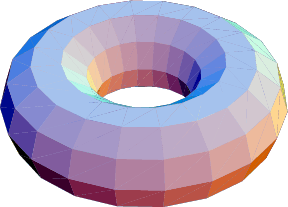
\includegraphics[height=1em]{torus}}}}}
\begin{frame}{Cohomology}
  \centering

  Is $\vcenter{\hbox{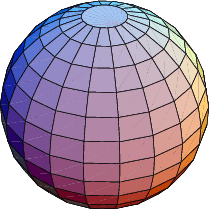
\includegraphics[height=0.1\textwidth]{sphere}}}$ homeomorphic to
  $\vcenter{\hbox{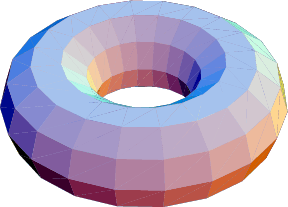
\includegraphics[height=0.1\textwidth]{torus}}}$? No:
  \begin{align*}
    H^0(\smallsphere,\ZZ) &\cong \ZZ &
    H^1(\smallsphere,\ZZ) &\cong 0 &
    H^2(\smallsphere,\ZZ) &\cong \ZZ \\
    H^0(\smalltorus,\ZZ) & \cong \ZZ &
    H^1(\smalltorus,\ZZ) & \cong \ZZ \oplus \ZZ &
    H^2(\smalltorus,\ZZ) & \cong \ZZ
  \end{align*}

  Basic tool: \bad{injective resolutions}
\end{frame}}

% \begin{document}

\begin{frame}{}%Injective and divisible abelian groups}
  \begin{block}{}
    \justifying
    \textbf{Def.}
    A group~$I$ is \hil{injective} iff for every injective map~\mbox{$A
    \hookrightarrow B$}, every map~$A \to I$ can be extended to a map~$B \to I$:

    \vspace*{-0.9em}
    \[ \xymatrix{
      A \ar@{^{(}->}[r]^{\forall i} \ar[d]_{\forall f} & B
      \ar@{-->}@/^/[ld]^{\exists \overline{f}} \\
      I
    } \]
  \end{block}
  \vspace*{-0.6em}
  \visible<6->{\small\justifying \ldots{} is \hil{Baer} iff extensions exist for all ideal
  inclusions~$\aaa \hookrightarrow \ZZ$.\medskip\par}
  \normalsize
  \pause

  \begin{block}{}
    \justifying
    \textbf{Def.}
    A group~$I$ is \hil{divisible} iff for every element~$x \in I$ and
    every~$n \in \NN_{>0}$, there is an element~$y \in I$ such that~$ny = x$.
  \end{block}
  \vspace*{-0.6em}
  {\small\emph{Examples.} $\QQ$, $\QQ/\ZZ$, $\ZZ(p^\infty)$.\par}
  \pause
  \vspace*{-0.3em}

  \grayline
  \begin{changemargin}{-2em}{-1.5em}
  \begin{enumerate}
    \only<1-4>{
      \item \badbox{\textsc{lem}+\textsc{zorn}} \\ Every divisible group is injective.
      \medskip
    }
    \only<5->{
      \item \normalnumber{a} \badbox{\textsc{lem}} Every divisible group has the Baer
      property. \\
      \normalnumber{b} \badbox{\textsc{zorn}} Every group with the Baer property is
      injective.
      \only<7->{\\ \small\emph{Proof.} Let~$f_0 : B_0 \to I$ be an extension.
      \visible<8->{\justifying Let~$x \in B$. \visible<9->{Set~\mbox{$\aaa = \{ n \in \ZZ \,|\, nx
      \in B_0 \}$}. \visible<10->{The map~$g : \aaa \to I,\,n
      \mapsto f_0(nx)$
      can be extended to a map~$\overline{g} : \ZZ \to I$. \visible<11->{
      Hence~$f_0$ can be extended to the map~$B_0 + (x) \to I,\, u + nx
      \mapsto f_0(u) + \overline{g}(n)$.}}}}}
      \medskip
    }

    \item\justifying There are models of~\textsc{zf} without
    nontrivial injective groups. [Blass]
    \medskip

    \item Every group embeds into a divisible group.
    \\\visible<4->{\emph{Proof.} If~$A = \ZZ\langle M \rangle/R$, then~$A
    \hookrightarrow \QQ\langle M \rangle/R$.}
  \end{enumerate}
  \end{changemargin}
\end{frame}

\begin{frame}{Logical sheaves}
  The set~$\NN$ is \hil{$\neg\neg$-separated} in that
  \[ \forall x,y\?\NN\_ \neg\neg(x = y) \Rightarrow x = y, \]
  but not a \hil{$\neg\neg$-sheaf}, which would mean
  \[ \forall S \subseteq \NN\_ \neg\neg(\text{$S$ singleton}) \Rightarrow
    \exists! x \? \NN\_ \neg\neg(x \in S). \]
  We can \hil{sheafify}:
  \[ \NN^+ = \{ S \subseteq \NN \,|\, \neg\neg(\text{$S$ singleton})
  \}/{\sim}\
  \text{with $S \sim T$ iff~$\neg\neg(S = T)$.} \]
  \grayline

  % Something about ¬¬-embedding, ideals of ℕ⁺

  \begin{block}{}
    \justifying
    \textbf{Prop.}
    The group~$(\QQ/\ZZ)^+$ has the Baer property.
  \end{block}
\end{frame}

\begin{frame}{There are enough Baer groups}
  \begin{block}{}
    \justifying
    \textbf{Def.}
    A \hil{local operator}~$\nabla$ is an operator such that
    \vspace*{-0.6em}
    \begin{align*}
      \varphi &\,\Longrightarrow \nabla\varphi \\
      \nabla\nabla\varphi &\,\Longrightarrow \nabla\varphi \\
      \nabla(\alpha \wedge \beta) &\Longleftrightarrow (\nabla\alpha) \wedge
      (\nabla\beta).
    \end{align*}
  \end{block}
  \vspace*{-0.6em}
  {\small\emph{Examples.} $\neg\neg$, \quad $\alpha_0 \Rightarrow \cdot$, \quad
  $\cdot \vee \beta_0$, \quad $((\cdot \Rightarrow \chi_0) \Rightarrow \chi_0)$.\par}
\end{frame}

\end{document}
